\documentclass[a4paper, UTF8]{ctexart}				%中文环境
%\documentclass{article}							%英文环境

%---------------------------宏包加载----------------------------
    \usepackage{amsmath}
    \usepackage{amssymb}
    \usepackage{amsthm}
    \usepackage{geometry}
        \geometry{left = 2.54cm, right = 2.54cm,
            top = 3.18cm, bottom = 3.18cm}			%页边距设置
    \usepackage{fancyhdr}
        \pagestyle{fancy}
        %\lfoot{\today}   							%左页脚
        \cfoot{\thepage}							%中页脚
        %\rfoot{}	 						 		%右页脚
        \setlength{\parskip}{0.5 \baselineskip}		%段距
    \usepackage{hyperref}  							%打开超链接
        \hypersetup{colorlinks=false}				%取消超链接颜色
    \usepackage{tikz}
    \usepackage{multirow}

%---------------------------标题设置----------------------------
    \title{并行计算作业}
    \author{林陈冉}
    \date{\today}

%---------------------------定理环境----------------------------
    \newtheorem{theo}{\bf 定理}[section]			  %新建定理环境, 标题为"定理", 以section为计数器标记
    \newtheorem{define}{\bf 定义}[section]
    \newtheorem{algo}{\bf 算法}
    \renewcommand{\proofname}{\bf 证明}			  %重命名定理环境, 标题为"证明"
    \numberwithin{equation}{section}				%以section为计数器标记公式

%-----------------------------正文------------------------------
\begin{document}									%开始正文
    \maketitle										%生成标题
    \paragraph{1}\quad 
        对于求矩阵maxmin问题, 即 
        \[
            y = \max_{1 \le i \le N} \min_{1 \le j \le N} a_{ij}
        \]
        显然, 这个问题的子任务为求每行的最小值. 我们按处理器数量 $p$ 分情况讨论子问题的合并.

        (1) 当 $p \le N$ , 我们让每个处理器计算 $N/p$ 行的最小值, 再算出这几行的结果中的最大值(当不能整除时, 如何取整会带来一定的问题, 实际上, 令 $N - p\lfloor N/p \rfloor$ 个处理器计算 $\lceil N/p \rceil$ 行, $p\lceil N/p \rceil - N$ 个处理器算 $\lfloor N/p \rfloor$ 行时, 各处理器的负载较为均衡). 求最小值算法显然是一个 $o(n)$ 的算法, 设每次次比较用时 $\alpha$ , 那么处理器的最大计算时间为
        \[
            T(cal) = \alpha ((N - 1)\lceil N/p \rceil + \lceil N/p \rceil - 1) = \alpha (N \lceil N/p \rceil - 1)
        \]

        计算完每行后, 要进行处理器间通信, 求各处理器的结果的最大值. 可以将这个过程分为很多轮, 每轮各处理器配对, 两两比较, 较大的进入下一轮比较, 不能凑对则轮空直接进入下一轮比较, 重复直至求出最大值, 示意图如下.
        \begin{center}
        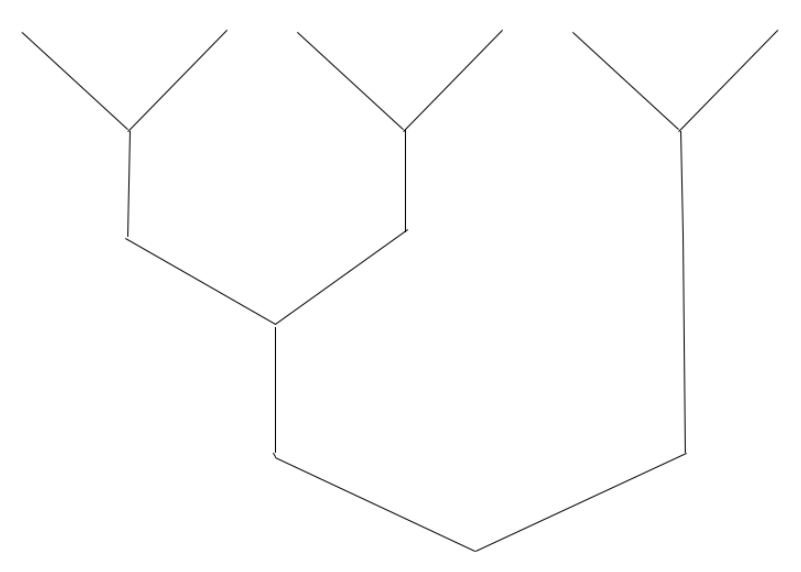
\includegraphics[width=7cm,height=5cm]{pic_2.png}
        \end{center}
        设两个处理器间单纯通信用时为 $\beta$ , 加上一次比较用时 $\alpha$ , 通信总用时为
        \[
            T(comm) = \sum_{i=1}^{\log p} (\alpha + \beta) p 2^{-i} = (\alpha + \beta)(p-1)
        \]

        整个过程总时间为
        \[
            T = T(cal) + T(comm) = \alpha N \lceil N/p \rceil + (\alpha + \beta) p - 2\alpha - \beta
        \]
        
        
        (2) 当 $p_0 \ge p > N$ ($p_0$ 是某个阈值, 后面会分析), 我们让 $p/N$ 个处理器去算每行的最小值(同样的, $N - N\lfloor p/N \rfloor$ 行由 $\lceil p/N \rceil$ 个处理器计算, $N\lceil p/N \rceil - N$ 行由 $\lfloor p/N \rfloor$ 个处理器计算时, 各处理器的负载较为均衡). 处理器的最大计算时间为
        \[
            T(cal) = \alpha (\lceil N/ \lfloor N/p \rfloor \rceil - 1)
        \]

        再考虑通信过程, 实际上这个过程还是在比较 $p$ 个处理器的结果, 用时没有发生变化
        \[
            T(comm) = (\alpha + \beta)(p-1)
        \]

        整个过程总时间为
        \[
            T = T(cal) + T(comm) = \alpha \lceil N/ \lfloor N/p \rfloor \rceil + (\alpha + \beta) p - 2\alpha - \beta
        \]

        实际上, 还应该有第三种情况, 处理器的数量应该有一个阈值 $p_0$ , 当 $p > p_0$ , 再按(2)中的方式分配处理器反而总时间会变慢. 忽略取整运算
        \[
            \frac{\partial T}{\partial p} = \alpha + \beta - \alpha N^2 p^{-2}
        \]
        令上式为0, 其解即为临界点 $$p_0 = \sqrt \frac{\alpha N^2}{\alpha + \beta}$$

        (3) 当 $p > p_0$ , 只取 $p_0$ 个处理器, 按(2)中方式参与运算 
        \[
            \begin{split}
                T(cal)     &= \alpha (\lceil N/ \lfloor N/p_0 \rfloor \rceil - 1)\\
                T(comm)    &= (\alpha + \beta)(p_0 - 1)\\
                T          &= \alpha \lceil N/ \lfloor N/p_0 \rfloor \rceil + (\alpha + \beta) p_0 - 2\alpha - \beta
        \end{split}  
        \]

    \paragraph{2}\quad 
        对于求积分问题, 即 
        \[
            y = \int_a^b f(x)dx = h\sum_{i=0}^{N-1} f(x_i),\quad x_i = ih,\quad h = (b-a)/N
        \]
        其子问题为求 $f(x_i)$ . 对于子问题的合并, 我们断言, $\exists p_0 < N$ , 使得当使用超过 $p_0$ 个处理器的时候用时反而变长, 分情况讨论.

        (1) 当 $p < p_0$ , 每个处理器计算 $N/p$ 个数的和(不能整除时, 分配方式类似上一题情况(1)), 设求每个 $f(x_i)$ 用时为 $\alpha$ , 单次求和用时为 $\beta$ , 则最大计算用时 
        \[
            T(cal) = \alpha \lceil N/p \rceil + \beta(\lceil N/p \rceil - 1) = (\alpha + \beta) \lceil N/p \rceil - \beta
        \]
        
        计算完成后, 类似上一题, 分多轮求总和, 每轮将各处理器结果两相加, 不凑整的数直接进入下一轮. 设处理器通信时间为 $\gamma$ , 则该过程通信时间为 
        \[
            T(comm) = \sum_{i=1}^{\log p} (\beta + \gamma) p 2^{-i} = (\beta + \gamma)(p-1)
        \]
        
        总时间为 
        \[
            T = T(cal) + T(comm) = (\alpha + \beta) \lceil N/p \rceil  + (\beta + \gamma)p - 2\beta - \gamma
        \]
        
        (2) 当 $p > p_0$, 只取 $p_0$ 个处理器, 按(1)中方式参与运算 
        \[
            \begin{split}
                T(cal)     &= (\alpha + \beta) \lceil N/p_0 \rceil - \beta\\
                T(comm)    &= (\beta + \gamma)(p_0 - 1)\\
                T          &= (\alpha + \beta) \lceil N/p_0 \rceil  + (\beta + \gamma)p_0 - 2\beta - \gamma
        \end{split}  
        \]

        考虑这个阈值 $p_0$, 忽略取整运算
        \[
            \frac{\partial T}{\partial p} = \beta + \gamma - (\alpha + \beta) N p^{-2}
        \]
        令上式为0, 其解即为临界点 $$p_0 = \sqrt \frac{(\alpha + \beta) N}{\beta + \gamma}$$
\end{document}										%结束正文
